%\documentclass[10pt,a4paper]{article}
\documentclass[twoside,openright]{scrreprt}
\usepackage[utf8]{inputenc}
\usepackage{amsmath}
\usepackage{amsfonts}
\usepackage{amssymb}
\usepackage{mathtools}
\usepackage{graphicx}
\usepackage{svg}

\usepackage{stackrel}
\usepackage{caption}
\usepackage{subcaption}

\usepackage[msc]{tugrazthesis}


\begin{document}
%--- INFORMATION FOR TITLEPAGE -------------------------------------------------

% Your name including previous academic degrees (optional argument sets a different \author{}):
\thesisauthor[Firstname Lastname]{Firstname Lastname, BSc}

% Title of your thesis (optional argument sets a different \title{}):
\thesistitle[Short Thesis Title]{Title and\\Subtitle\\of the Thesis\\(up to 4 Lines)}

% Date of completion (optional argument sets a different \date{})
\thesisdate[ ]{Month Year}

% Supervisor headline (select male/female/plural version)
\supervisortitle{\germanenglish{Betreuerin/Betreuer}{Supervisor}}

% Supervisor info
\supervisor{%
  Markus Koch, academic degrees of supervisor\\
  up to 2 lines

  Institute of Experimental Physics\\
  up to 2 lines

  %optional extra information (second advisor, name of faculty, etc.)\\
  %up to 2 lines
}

% Academic degree achieved with this thesis, according to your curriculum (check curriculum and select male/female version):
\academicdegree{Diplom-Ingenieur}

\chapter{Devices and Setup}



Part of the experimental objective was to extend the range of the transient absorption microscope (TAM) into the UV range via SHG of the probe NOPA output. With the extension a wavelength range of 250 nm to 940 nm, with a gap between 470 nm and 500 nm, is available for probing the sample.\newline
To achieve this range a few optics, most notably the achromatic objectives used to image the sample, had to be exchanged for optics non absorbing in the UV.
\section{Regular Transient Absorption Microscope Setup}\label{RegTAM}
A short description of the experimental setup for the Transient Absorption Microscope (TAM), as it was before attempting an extension to higher photon energies follows. For further details see previous work (cite robert master thesis)\\
As a laser source a PHAROS femtosecond laser by Light Conversion is used with an output of 400 µJ at 20 kHz with a pulse length in the range of ....? The output is evenly split between two Orpheus Non-Collinear Optical Parametric Amplifiers (NOPAs), where one is setup with second harmonic (2H) for the pump pulses (650 nm - 940 nm) and the other is setup with third harmonic (3H) for the probe pulses (500 nm - 940 nm). Long term output power stability is mainly important for the pump pulse, which is why the setup, including the compressor the PHAROS, is optimized for maximum stability of the 2H NOPA. Meanwhile having little shot to shot fluctuations is important in all cases. PHAROS is the most reliable part of the setup, with exception of the compression setting which may need adjusting every once upon a while.\\

The light following the pump path goes through several apertures and ND filters, which may be absorptive glass filters or metal coated reflective filters which may also be gradient filters for linear adjustability, until the beam reaches the linear delay stage, which uses a Newpot LTA-HS actuator. The beam path is then led through the chopper by the use of a roughly 1:1 telescope around it, which blocks every second pulse leaving a half frequency signal for the pump. The chopper is synchronised to a signal output of PHAROS, which allows for setting a delay such that there is just a binary on and off modulation of the pump, compared to a partial chopping of beams at full frequency. After passing through a lambda half wave plate the beam enters the common path in the cage with the sample.

The probe beam has the same treatment of apertures and ND filters, including a variable reflective one, and goes through a $\mathrm{\lambda/2}$ plate until it reaches the common path.


For detection of the transient signal a custom made detector based on Hamamatsu S1336-8BQ Si photodiode is used in combination with an analogue long pass amplification circuit stretching the signal such that it can be measured with a picoscope 5442D. For all measurements detector "A" was used. The diode is fit for measurements in the wavelength range of 190-1100 nm. The actual quantum efficiency change over the spectral range does not matter in detail, as the variation over the spectral range is slow and for the spectral range of a probe setting does not exceed 10\% change at any point.

\section{UV extended Transient Absorption Microscope Setup}
This section will address the issues addressed with the extended setup as well as attempted solutions and the final changes to make it work.

\begin{figure}[h]
\centering
\includegraphics[width=0.9\linewidth]{images/ComponentLibrary_svg/TAM-SetupUV.png}
\caption{UV extended TAM\\Pump adjustable for 650 nm to 940 nm
\\Probe adjustable between 500 nm and 940 nm with the option of separate range of 250 nm and 470 nm via SHG crystal\\
SHG stage shown including optional filters to remove white light from NOPA (ahead of SHG crystal) and fundamental wavelength of SHG (after SHG crystal)\\ Cage setup in further detail in fig. \ref{Fig:CageSetup}}
\end{figure}

\begin{figure}[h]\label{Fig:CageSetup}
\centering
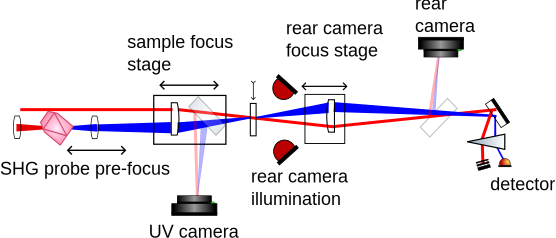
\includegraphics[width=0.9\linewidth]{images/ComponentLibrary_svg/TAM_Setup-SHGandDetector.png}
\caption{Detail view of new components in TAM\\ Ahead of first show probe lens white light remainder from NOPA may be filtered and after the second lens the fundamental may be filtered\\
Rear camera shown as coupled out of the standard path, however it is advised to instead have the rear camera in the standard detector path and only insert the mirror coupling into the mirror when doing measurements.}
\end{figure}

\subsection{Cage setup}
To accommodate the lower wavelengths the objectives have to be exchanged for wavelengths below 350 nm, where absorption reduces the transmission of the objective combination severely. Furthermore only one of the objectives is rated down to 350 nm raising the question of if their achromacity still is a viable assumption.\newline
The objectives are replaced with  uncoated 125 nm plano-convex UV fused silica (UVFS) lenses from EKSMA\footnote{?110-1216E?}, with the convex side placed such that the collimated beam enters or exits the convex side. This means that the planar sides of the lenses point towards the sample as can be seen in fig. \protect\ref{Fig:CageSetup}. This is done to reduce spherical aberration.
\newline
The plano-convex lenses are neither apochromatic nor achromatic and thus exhibit chromatic aberration, leading to an issue that will be addressed in \ref{SHG-Stage-desc}. \newline

\subsection{Second Harmonic Generation stage}\label{SHG-Stage-desc}
The Second Harmonic Generation (SHG) stage addresses multiple issues. 
\begin{itemize}
\item The 3H NOPA used for the probe beam does not supply high enough power to allow for stable SHG over the entire output wavelength range of the NOPA without a focusing element increasing the power locally within the crystal. 
\item The chromatic aberration or focus shift within the cage system means that a degree of freedom on the focus of the probe needs to be included as to allow for adjustments to the pointspread function of the probe.
\end{itemize}


The solution to these issues is an adjustable telescope of biconvex lenses, of which the second lens has to be UV transmissive. To achieve a stable second harmonic generation (SHG) a telescope was built with two spherical lenses. The front lens is a 85 mm lens in a mount adjustable for horizontal and vertical displacement orthogonal to the beam path and the rear lens is a 75 mm UVFS lens on a linear stage, to provide a degree of freedom for the focus of the probe beam, which is necessary to account for the achromacity of the extended setup.
\subsubsection{Operation}
\paragraph{Setting up}
The task of setting up the SHG stage is non trivial regarding proper alignment and linear stage positioning, such that the ~5 cm of movement are sufficient to adjust for the chromatic aberration within the targeted wavelength range for probe. This task often ends up being trial and error in correspondence to checking multiple wavelengths. The cage lenses have to be in their correct positions first.\newline
Irises etc are beneficial if there is a working setup.\newline
Use irises to shape the probe beam to an acceptable Gaussian shape while avoiding diffraction effects. Optimally the incoming beam is level with the table, since any inclination will introduce an astigmatism? depending on the rear lens position.\newline
Begin with the first lens in the path leaving enough space for the linear stage and the SHG crystal to the next static optic. Set lens centered regarding beam. Use the irises in front of the lens to adjust the reflection on the lens surface to return the exact incoming beampath.\newline
Place the rear stage lens and once again adjust for center position. One may again use the reflection and additionally the transmitted beam to tell if the stage is parallel to the beam path. The center of the beam should not move when translating the stage and the expansion of the beam diameter should be as symmetric as possible. Adjusting via the reflection is not such a clear indication of alignment here, as there are multiple convex surfaces in play at this point, leading to multiple focal beams, what may not be in full accordance with each other. For this usually it was chosen to get the highest intensity spot, which refers to the final glass/air surface of the second lens, in the incoming beam path. This spot is also focused, which makes adjustment easier.\newline
Finally one can adjust mirrors after the stage to get an image on the camera again, as even relatively minute changes in alignment will lead to some beam offset and change in direction. Translating the stage then will give an indication of how well the SHG stage is set up in regards to astigmatism which can be seen as non symmetric expansion of the beam. However beware that the mirror outcoupling in the cage also influences the way a change in focus is experienced, due to deviations from an orthogonal inclination angle to the sensor.
\paragraph{For measurements}
To find SHG intensity approach from the incoming beam direction and adjust SHG crystal until sufficient output power is achieved.\newline
Adjust the linear stage such that there is no lateral movement. The current stage slide is mounted in a way that can rotate a bit if force is applied at the corners. It may be necessary to do this and have the stage "snap back" to make sure it will not move during the measurement. This can be checked after the measurement by checking the overlap again.
\subsection{Detector Setup}
The detectors themselves are the same as described in Robert Schwarzl's master thesis.\cite{Schwarzl2021} For the measurements detector A was used at all times in combination with a picoscope 5442D. An equal sided, UV translucent, prism is inserted to remove any remainders of the fundamental probe wavelength at the detector. To improve this separation an extra iris may be used immediately in front of the detector.\\
The prism should be placed such that the angle between pump and probe is further increased, as this can help reach full pump rejection without any other filters or beamblocks involved. For each change of the probe the mirror coupling into the prism should be adjusted for maximum intensity of the probe on the detector, which can be monitored using the fourierDetector() matlab program.\\
The detector has a maximum peak to peak voltage (Vpp) of approximately 3 V, which means that the Vpp should be kept below this value to avoid response problems and thus systematic errors in the measurement.
\subsection{Adjusting overlap without achromatic optics}
One of the main issues that had to be addressed was the change from achromatic objectives to uncoated plano-convex lenses within the cage.\newline
This is emphasized especially by plotting the wavelength dependence of the focal length as defined by the lensmaker equation for the lenses used:
\begin{equation}
\frac{1}{f} = (n-1) \left[\frac{1}{R_1} - \frac{1}{R_2} + \frac{(n-1)d}{n R_1 R_2}\right]
\end{equation}
\begin{figure}[h]
\centering

\begin{subfigure}[b]{0.45\textwidth}
\centering
\includegraphics[width =\textwidth]{images/DispersionUVFS.png} 
\caption{Refractive index of UV fused silica glass\cite{Malitson:65}}
\end{subfigure}
\hfill
\begin{subfigure}[b]{0.45\textwidth}
\centering
\includegraphics[width =\textwidth]{images/ChromaticAberration.png} 
\caption{Chromatic focal shift}
\end{subfigure}

\caption{Refractive index change and focal shift for UV fused silica plano-convex lenses used in cage setup}
\end{figure}

Furthermore the depth of focus may be visualized by plotting the beam waist diameter over distance from the focal point for several relevant focal lengths in fig. ....

The change of the depth of focus (DOF) and thus the change in beam waist diameter for a specific distance from the focal point of the corresponding wavelength decreases for higher photon energies.

\begin{figure}[h]
\centering
\begin{subfigure}[t]{0.42\textwidth}
\centering
\includegraphics[width =\textwidth]{images/BeamWaist_Wavs_2.5mm.png} 
\subcaption{Beam waist for wavelengths at \mbox{2.5 mm} input beam width}
\end{subfigure}
\hfill
\begin{subfigure}[t]{0.42\textwidth}
\centering
\includegraphics[width =\textwidth]{images/BeamWaist_inputWidth_653nm.png} 
\subcaption{Beam waist over input beam width at 653 nm}
\end{subfigure}
\\
\begin{subfigure}[t]{0.5\textwidth}
\includegraphics[width =\textwidth]{images/DOFintensity_inputWidth_653nm.png} 
\subcaption{Maximum radiance intensity relative to maximum intensity in focus depending on input beam width at 653 nm[check if this assumption is correct]}
\end{subfigure}
\caption{Changes of Gaussian beamprofile width and intensity for cage lenses}
\end{figure}

This issue is of fundamental nature and a few attempts were made until the final solution in \ref{SampleMirrorCamera} was found.
\subsubsection{Regular Focusing after Cage}\label{regRearFocus}
This is the option used for the regular TAM setup as described in \ref{RegTAM}. The last mirror in front of the detector is simply removed to reveal a camera behind it. The rear cage objective is focused onto this camera using white light from an LED torch or similar lightsources in transmission. Afterwards the front objective is moved such that a satisfactory pointspread function of the beam is seen from the camera sensor.\\ 
This is sufficient as the achromatic objectives allow a very similar focus for all wavelengths between 400 nm and 940 nm. The rear objective simply projects the pointspread function of the beams in the plane of the sample to which it was focused to, while moving the front objective adjusts the part of the focusing beam cone, and thus the size of the slice of the beam, which interacts with the sample. This is working for both pump and probe.\\
Since the focal length of the lenses varies wildly in the UV this is not an option for the UV extension.
\subsubsection{Dummy Conversion Sample}
An idea was to use a "dummy" sample acting as a screen to then be imaged onto the camera in the rear using the lens. This method has several requirements:
\begin{itemize}
\item The screen needs to allow for diffuse imaging of the sample without disturbing the beamshape too much.
\item Any UV or near UV light needs to be converted to the visible region, where the focal length difference becomes negligible.
\end{itemize}

The requirement for diffuse imaging is simple. Any collimation or focusing action of the beam needs to be lost to actually image the sample plane, where the "dummy" is placed at. The requirement is less stringent for wavelengths close to a chosen wavelength to which the setup would be calibrated to, as the lenses would image the beam fine for that wavelength.\\

For the issue of UV conversion a few attempts with different dyes and paper were made, which showed variable success as to their luminescence.\\
Generally paper combined with orange gel marker (Stabilo No. 70/40) seemed to work best
Paper soaked with wax to increase transmittance and smooth out scattering alone did not work particularly well unless combined with text marker. Marker has to be applied ahead of the wax and on the other side of the paper, from where the wax will be applied. (I am considering just throwing this all out, though having an off hand comment shouldn't be too bad) 

Using a microscope slide with gelled, specifically at room temperature evaporated, Stabilo marker (No. 70/40) turned out to have decent conversion efficiency, but lacks any diffusivity. This could work, based on adjusting the cage setup to the pump wavelength, so it is correctly imaged. However at that time the rear focus was still set with white light instead of 653 nm pump adjacent light, which would not have allowed for this method. Also this leads to problems as soon as the probe light has long enough wavelengths to simply transmit through the glass slide. It would need to be filtered, which at the time was not possible as longpass filters were not available to us. Another unanswered question is the emission spectrum of the marker gel. (lab notes  starting in june)\\
Surprisingly the frontal focus point found with this projection method coincides well with the finally used frontal focus point. Consider that the projection screen may not be spaced entirely correctly though. CHECK THICKNESS
Overall the attempted projection screen method did not seem viable and thus was not pursued further. A main disadvantage, apart from problems with wavelength conversion, is that in the best case the scattering applies a strong averaging to the beam pointspread function, which does not allow for detection of deviations of the beam shape from a Gaussian distribution. Unless a very consistent and fine scattering projection screen with good conversion to a specific wavelength band close to the pump is found it just is infeasible.


\subsubsection{Sample mirror path}\label{SampleMirrorCamera}
The option that finally won out is decoupling the beams after the frontal cage lens and imaging onto a camera that is in the mirror plane of the sample surface. This method requires a method for consistent placement of the mirror within the cage and a way to move the camera into the mirror plane of the sample.\\
\paragraph{Method}
The rear lens is set to image the sample plane onto the camera as described in \ref{regRearFocus} with a pump adjacent wavelength used to illuminate the sample. This is done to be able to use the pump beam as a reference for the cage system, as the front focus for the sample and the rear focus for the camera are both calibrated using a wavelength with very little chromatic focal shift from it.\\
A two step process is then used to get the position of the camera in the mirrored sample path correct:
\begin{enumerate}
\item Adjust the frontal camera distance so, that the pump beam profile is right before inversion, due to passing through the focal point. Inversion being the outer features of the beam profile passing through the center. The intensity still rises a bit beyond that point. Attention has to be paid to not go into inversion, which is hard to tell by eye. Later on this could be done by comparing the fitted intensity value/FWHM of the beam profile as long as the pump beam did not change. Placement of OD filter in front of camera or in front of cage does matter, swapping the position changes the beam profile.
\item Set the probe to the same or an adjacent wavelength to the pump and setup overlap using the rear camera. Due to beampaths and thus spherical abberation this may be a tedious process and not completely accurate. Check the overlap on the frontal camera by moving the camera back and forth and observing if the beams cross through their centers. If that is the case the pump probe overlap should be given optimally and the frontal camera can be set to the optimum position of this overlap. Take reference TA measurements to if possible to check if there is an improvement from the purely DMK set position.
\end{enumerate}
\paragraph{Setup}
Former is solved by a 45 degree mirror insert for the cage, which was designed to rest on top of the cage system rails. This drop in mirror mount was 3d printed for adjustability and has proven to be consistent enough to allow for this method to work. \\
An advantage of PLA as opposed to aluminium with the negative of the rails cut into it is that it allows proper sliding into place, whereas aluminium "gripped" onto the rails making it hard to get consistent placement. This may be improved by cutting the rail negative even slightly bigger. However this still presents one with the problem of how to mount the mirror to the mount. Super glueing  the mirror to the Al mount was attempted for a quick trial, but this proved to not be a long lived connection.\\
The 3d printed mount can be seen in fig. ....
Considerations regarding use of rubber bands or 3d printed fittings were made, however it turns out just by moving the mirror drop-in mount against a solid surface, such as one of the cage plates holding the rails, is sufficiently reproducible for the sensor resolution of the camera used. (alternatively also reference the change in beam diameter according to rayleigh length etc)\\

The lighting for imaging the rear sample onto the camera via the rear lens is done using a ring light with 4 LEDs, which have a spectral intensity distribution close to the targeted pump beam. The spectrum can be seen in fig. ...\\
It has proven beneficial to illuminate so that a only scattered light is detected, as this equivalent to darkfield microscopy this should improve contrast. As this means reduced total intensity any light not scattered by the sample or reflected from nearby surfaces needs to be blocked. For this carton is placed around the rear cage rails, cutting away any light reflected from the sample mount.
%The LEDs are mounted onto a square aluminium frame and are angled towards the sample to illuminate it evenly. To properly setup the focus light that not passing through the lens has to be minimized or contrast will be lost. To focus properly a small scratch is introduced to the edge of the sample, which allows better contrast for focusing as well and allows to focus closer to the center to the layer than to the top or bottom of the layer. (eh questionable, think better)


\chapter{Software}
\section{Overlap Compensation}
Opposed to the old setup, where the achromatic objectives guaranteed relatively consistent overlap of pump and probe, the UV setup has the need to correct the variation between the single measurements, since the diffraction of the dispersive elements in the probe path varies strongly in the UV range and any compensation via the telescope will be imperfect.\newline
Relevant for this are the beam size of the probe as well as the overlap of the pump and the probe beam in the sample. Variations in those parameters are induced by change of the beamshape due to SHG generation, imperfect alignment of the SHG telescope and correction of the chromatic aberration for different wavelength settings of the probe.\newline

\subsection{Beam Characterisation}
The python class ArtFit has some options to check for the validity of the data used. Since the data is saved in a raw format, however it is cut and thus an offset for the ROI has to be accounted for. \footnote{NOTE: FOR ARTRAY VER 1.3 CHANGE SO METADATA OF ROI OFFSET IS SAVED, ALSO OF BACKGROUND FILE: may not work like I hoped}

ArtFit may parse 3 different input types: (think of something different, not meaningful like this)
\begin{enumerate}
\item Quick plotting of raw data:\\
With a path to a raw data file and an optional bool value, which is used to tell the program to use the standard size of 1280x720 instead of a square pixel array size deduced from total number of entries. Plots the beam intensity profile without any processing.
\item Single beam profile with background subtraction: \\
Loads a JSON characterising the background file, including a set offset of ROI, the path for the beam profile to be loaded and a width for fitting.
\item Two beam profiles with background subtraction: \\
ROI offset has to be identical and is again defined by a JSON file with background location.
\end{enumerate}

To get meaningful data for correction of data the pump power has to be set using setPumpPower() and the scale can optionally be overwritten from the background file with setScale(). Fitting is done by calling plainFit(id), where id = 1 for probe (first path handed over) and id = 2 for pump (second path).

Some options to show 
\begin{itemize}
\item plotComp()\\
Shows an intensity contour plot of both beams on top of each other. If only one beam file is loaded only one is shown. Also shows the fitted intensity slices on top of each other for both pixel array axis. Returns an overlap value corresponding to what is given by the liveFitting program described in section \ref{Sec:LiveFitting}.
\item plotGauss()\\
Plots the intensity profile of the beams, if both are given, separately with an overlayed contour plot of the fits, to allow to ascertain the validity of the fit. Needs to have already fitted data with plainFit() to show the Gaussian distribution. Fitted data may be printed to console by setting printData = True for the options. The intensity profile is shown by default without background subtraction and can be shown with subtracted background by handing over a boolean. The fits are always done with subtracted background, the profile just is not shown background subtracted by default.
\end{itemize}
\subsection{Correction Factor}
The correction factor aims to equilibrate the dOD of the given pump-probe overlap to one where the pump is constant in radiance over the entire probe area or in a physical description is infinitely larger than the probe beam.
Thus for very high $\mathrm{\frac{\sigma_{Pump}}{\sigma_{Probe}} \rightarrow \infty}$ the correction factor tends to 1, which is the smallest value.\\
The factor is calculated from the Gaussian intensity distributions as seen in eq. \ref{CorrFactorGaussians}, of which the derivation is shown in section \ref{GaussiansDerivation} or in Bromiley\cite{Bromiley2014}, which was used to check correctness. The enumerator is the integral over essentially the probe intensity with the constant factor of the maximum pump intensity 
\begin{equation*}
I_{pump}^* = c^* = max(I_{pump}(x)) = \frac{1}{\sqrt{2\cdot\pi}\cdot\sigma_{pump}}
\end{equation*}, which is 1 due to the intensity taken as a Gaussian or normal distribution. The denominator is the integral over the product of the fitted normal distributions of pump and probe beams called $\mathrm{S_{12}}$.

\begin{equation}\label{CorrFactorGaussians}
C = \dfrac{\int I_{pump}^*\cdot I_{probe}(x) \;dx}{\int I_{pump}(x)\cdot I_{probe}(x) \; dx} = \dfrac{c^*\cdot \int I_{probe} dx}{S_{12}} = \dfrac{c*}{S_{12}}
\end{equation}

\begin{gather}
I_1(x)\cdot I_2(x) = I_{12}(x) = S_{12}\cdot \frac{1}{\sqrt{2\pi}\sigma_{new}} exp\left(-\frac{\left(x-\mu_{new}\right)^2}{2\cdot\sigma_{12}^2}\right)\label{GaussianProduct}\\
\int I_{12}(x)\; dx \coloneqq S_{12} \cdot 1\\
\sigma_{new} = \dfrac{\sigma_1 \cdot \sigma_2}{\sqrt{\sigma_1^2+\sigma_2^2}}\\
\mu_{new} = \dfrac{\mu_1\sigma_2^2 + \mu_2\sigma_1^2}{\sigma_1^2 + \sigma_2^2}
\end{gather}



\begin{equation}
S_{12} = \dfrac{1}{\sqrt{2\pi\left(\sigma_1^2+\sigma_2^2\right)}}\cdot exp\left(-\dfrac{\left(\mu_1 - \mu_2\right)^2}{2\cdot \left(\sigma_1^2+\sigma_2^2\right)}\right)
\end{equation}
A few examples of the behavior of the correction factor are shown in fig.

Furthermore to have all relative $\mathrm{\Delta OD}$ values be directly comparable, the correction factor is divided by the peak radiance value.

\begin{table}[h]
\begin{tabular}{lll}
$\Delta \mu$ / $\sigma$               & $\dfrac{\sigma_{pump}}{\sigma_{probe}}$ / 1 & Correction Factor                                                                                                \\ \hline
0                                     & 1                                           & $\sqrt{2}$                                                                                                        \\
$\Delta\mu$                           & 1                                           & $\sqrt{2} exp \left( \dfrac{\Delta \mu ^2}{4}\right)$                                                             \\
$\approx \sigma$                      & 1                                           & $\sqrt{2}exp\left(\dfrac{1}{4}\right)$                                                                            \\
$\infty$ & 1                                           & $\sim$ exp$\left(\Delta mu ^2 \right)$ \\
$2\cdot\sqrt{2 ln(2)}\sigma$       & 1                                           & $\sqrt{2}exp(2ln2)\approx 5.6$                                                                                    \\
0                                     & 3                                           & $\sqrt(\dfrac{9+1}{9}) \approx 1.054$                                                                             \\
0                                     & 1/3                                         & $\sqrt(\dfrac{9+1}{1}) \approx 3.2$                                                                               \\
0                                     & 1/2                                         & $\sqrt(\dfrac{4+1}{1}) \approx 2.2$                                                                               \\
0                                     & 2                                           & $\sqrt(\dfrac{4+1}{4}) \approx 1.12$                                                                             
\end{tabular}
\end{table}
\subsection{Artray-LiveFitting}\label{Sec:LiveFitting}
As the Artray $\mathrm{ARTCAM-092UV-WOM}$ could not be interfaced with matlab using the webcam library a C\# program was created based on the manufacturers example program.
Issues with our system are that for our specific camera or system setup a periodic variation of low intensity signal is reported by the C\# based program, while this periodic variation is missing in the official software. Attempts were made to troubleshoot this in correspondence with the manufacturer, who were very forthcoming in the matter, but it could not be solved so far. To overcome this problem a simple background subtraction has been devised as sufficient, as the variation seems to be constant over time. The background has been recorded with the lens cap on at an exposure of 15 ms, which was chosen after comparing the subtracted quality output of 0.3 ms, 15 ms and 100 ms. 
\newline
For all measurements included here version 1.2 was used. The  ALGLIB software package is used and (version number)\footnote{ALGLIB for C\# licensed as per GPL 2} for fitting a Gaussian to the beamshape.\\
In version 1.2 the relevant fitting parameters are returned as a numeric overlap integral based on the Gaussian beamshapes. In this version it is still calculated numerically from the fits, however it can be rebased into an analytical form as per eq. \ref{GaussianProduct} which describes the product of two Gaussians.
\begin{equation}
overlap = \int \sqrt{f_1(x)*f_2(x)}dx =  \sqrt{\frac{2 \sigma_1^2\sigma_2^2}{\sigma_1^2+\sigma_2^2}}\cdot exp\left(-\frac{\left(\mu_1-\mu_2\right)^2}{4\cdot \left(\sigma_1^2 + \sigma_2^2\right)}\right)
\end{equation}
This is calculated separately for both axis of the pixel array and then multiplied for a final value. (CHECK IF THAT IS ACTUALLY FINE AND PROVE IT WITH SIMULATION, same question as for correction factor)
This is not directly related to correction factor calculated within the python program to make everything comparable, but is more of a measure of how similar the beams are, which is why only the normal distributions are used without an intensity modifier, thus both beams are weighted identically. \\
This is reasonable as the best results for the correction factor are achieved when pump and probe beams are similar in size. This overlap integral returns a maximum value of 1 when the beams are identical and falls off quickly if the intensity maxima are shifted and slowly if the FWHM of the beams is different.\\

\chapter{Examination of reliability}
Some tests have been done to ascertain the validity and stability of the corrections devised for the UV extended TAM.






\chapter*{Used materials}
\begin{tabular}{|c|c|c|}
\hline 
Type & Device & SN \\ 
\hline 
lambda/2 & 400 nm - 800 nm; 690 nm - 1200 nm AHWPM10-986 & • \\ 
\hline 
Wire grid polariizer & WP25W-U5 & - \\ 
\hline 
UV-camera & Artray 092UV-WOM & • \\ 
\hline 
red LED & 658 nm & • \\ 
\hline 
LED driver & LT3080 based 12V input& • \\ 
\hline 
Prism & unknown; 300 nm permissive & • \\ 
\hline 
Camera & DMK 42AUC03 & • \\ 
\hline 
Power meter & Field Mate + head & - / 1019L08R \\ 
\hline 
X-Y stage actuators & Z825B with Thorlabs Kinesis Cube & • \\ 
\hline 
\end{tabular} 

\chapter{Derivations of formula}
\section{Produkt of two Gaussians}\label{GaussiansDerivation}
This calculation has been cross checked with Bromiley.

\begin{gather}
\begin{split}
G_{12}(x) & =  G_1(x) \cdot G_2(x) \\ 
& = \frac{1}{2\pi \sigma_1 \sigma_2}
exp\left(-\frac{1}{2}\left[\frac{\left(x-\mu_1\right)^2}{\sigma_1^2} + \frac{\left(x-\mu_2\right)^2}{\sigma_2^2} \right]\right)
\\
& = \frac{1}{2\pi \sigma_1 \sigma_2} exp \left(-\frac{1}{2\sigma_1^2 \sigma_2^2} \left[
\sigma_2^2 \left(x^2 - 2 \mu_1 x + \mu_1^2 \right) + 
\sigma_1^2 \left(x^2 - 2 \mu_2 x + \mu_2^2 \right)
\right] \right)
\\
& = \frac{1}{2\pi \sigma_1 \sigma_2} exp \left(-\frac{1}{2\sigma_1^2 \sigma_2^2} \left[
x^2(\sigma_1^2+\sigma_2^2) - 2x(\mu_1\sigma_2^2 + \mu_2\sigma_1^2) + (\sigma_1^2 \mu_2^2 + \sigma_2^2 \mu_1^2)
\right] \right)
\end{split}
\\
\sigma_{12} \equiv \sqrt{\sigma_1^2+\sigma_2^2}
\\
G_{12}(x) = \frac{1}{2\pi \sigma_1 \sigma_2} exp \left(-\frac{\sigma_{12}^2}{2\sigma_1^2\sigma_2^2}\left[
x - 2x\frac{\mu_1\sigma_2^2+ \mu_2\sigma_1^2}{\sigma_{12}} + \frac{\sigma_1^2\mu_2^2 + \sigma_2^2\mu_1^2}{\sigma_{12}}
+ \epsilon - \epsilon
\right]\right)
\\
\left(\frac{\mu_1 \sigma_2^2 + \mu_2\sigma_1^2}{\sigma_{12}^2}\right)^2 \stackrel{!}{=} \frac{\sigma_1^2\sigma_2^2 + \sigma_2^2\mu_1^2}{\sigma_{12}^2} + \epsilon
\\
\begin{split}
\epsilon \cdot \sigma_{12}^4  & = \mu_2^2\sigma_1^4 + \mu_1^2\sigma_2^4 + 2\mu_1\mu_2\sigma_1^2\sigma_2^2 - \sigma_1^2\mu_2^2(\sigma_1^2+ \sigma_2^2) - \sigma_2^2\mu_1^2(\sigma_1^2+ \sigma_2^2)\\
& = - (\mu_1^2\sigma_1^2\sigma_2^2 + \mu_2^2\sigma_1^2\sigma_2^2 - 2 \mu_1\mu_2\sigma_1^2\sigma_2^2)\\
& = - \sigma_1^2\sigma_2^2(\mu_1-\mu_2)^2
\end{split}
\\
G_{12}(x) = \frac{1}{2\pi\sigma_1\sigma_2}\cdot exp\left(- \frac{\sigma_{12}^2}{2\sigma_1^2\sigma_2^2\sigma_{12}^4}\sigma_1^2\sigma_2^2\left(\mu_1-\mu_2\right)^2
\right) \cdot
exp\left(-\frac{\sigma_1^2+\sigma_2^2}{2\sigma_1^2\sigma_2^2} \left[x - \frac{\mu_1\sigma_2^2+\mu_2\sigma_1^2}{\sigma_{12}^2}\right]^2 \right) \\
\sigma_{new} = \frac{\sigma_1\sigma_2}{\sigma_{12}}
\\
\mu_{new} = \frac{\mu_1\sigma_2^2+ \mu_2\sigma_1^2}{\sigma_{12}^2}
\\
\begin{split}
G_{12}(x) & = \frac{1}{\sqrt{2\pi}\sigma_{new}}\frac{\sigma_{new}}{\sqrt{2\pi}\sigma_1\sigma_2}\cdot exp\left(- \frac{\left(\mu_1-\mu_2\right)^2}{2\sigma_{12}^2}\right) \cdot
exp\left(-\frac{\left(x-\mu_{new}\right)^2}{\sigma_{12}^2}\right)\\
& = S_n \cdot \frac{1}{\sqrt{2\pi}\sigma_{new}} \cdot exp\left(-\frac{\left(x-\mu_{new}\right)^2}{2\sigma_{new}^2}\right)
\end{split}
\end{gather}



\bibliographystyle{ieeetr}
\bibliography{MasterThesisPrep}

\end{document}
